\documentclass[11pt, aspectratio=169]{beamer}

\usepackage[utf8]{inputenc}
\usepackage{tikz}
\usepackage[english]{babel}
\usepackage{svg}
\usepackage{eurosym}
\usepackage{subfig}
\usepackage{pgfgantt}
\usepackage[export]{adjustbox}
\usepackage{float}

% \usepackage[table]{xcolor}

\usepackage{color, colortbl}
\definecolor{Gray}{rgb}{0.8,.8,.8}

\usepackage{soul}
\usepackage{eurosym}

%\usepackage[shortlabels]{enumitem}
\usepackage[font=scriptsize,justification=centering]{caption}
\usepackage{movie15}
\usepackage{tikz}
\usetikzlibrary{arrows,shapes,positioning,shadows,trees}
\graphicspath{{figures/}}

%----------------------------------------------------------------------------------------
%   TITLE PAGE INFORMATION.
%----------------------------------------------------------------------------------------
\author{S. Björk, J. Hooper, J. M. Inga, H. Magnusson, A. Śmiałek}
\title{InfraRed Imaging of astronomical targets with a Stabilised Camera}
\subtitle{IRISC}
\institute{Luleå University of Technology, Kiruna}
\date{19 August 2019}
%\subject{} 

%----------------------------------------------------------------------------------------
%   SETUP LAYOUT.
%----------------------------------------------------------------------------------------
\usepackage{theme/beamerthemeWarsawLTU}
%\usetheme{Warsaw}


\begin{document}
%----------------------------------------------------------------------------------------
%   TITLE PAGE.
%----------------------------------------------------------------------------------------

{\setbeamertemplate{logo}{}
\begin{frame}
\titlepage
\begin{tikzpicture}[remember picture,overlay]
    \node[xshift=13cm,yshift=-1.025\textheight,anchor=north west] at (current page.north west){%
    
\includegraphics[width=2cm]{theme/LTU_logo.jpg}};
\end{tikzpicture}
\end{frame}
}

%----------------------------------------------------------------------------------------
%   TABLE OF CONTENTS.
%----------------------------------------------------------------------------------------
\begin{frame}[t]{Table of Contents}
\vspace{-0.3cm}
    \begin{columns}[t]
        \begin{column}{.5\textwidth}
            \tableofcontents[sections={1-2}]
        \end{column}
        \begin{column}{.5\textwidth}
            \tableofcontents[sections={3-5}]
            \vspace{-.2cm}
            \tableofcontents[sections=6,hidesubsections]
        \end{column}
    \end{columns}
\end{frame}

%----------------------------------------------------------------------------------------
%   INTRODUCTION / EXPERIMENT OVERVIEW.
%----------------------------------------------------------------------------------------
\section{Experiment Overview}



%----------------------------------------------------------------------------------------
%   SYSTEM.
%----------------------------------------------------------------------------------------
\section{System}
%   CONSTRUCTION. -----------------------------------------------------------------------
\subsection{Mechanical Design}
\begin{frame}{Mechanical setup}
	\begin{figure}
		\centering
		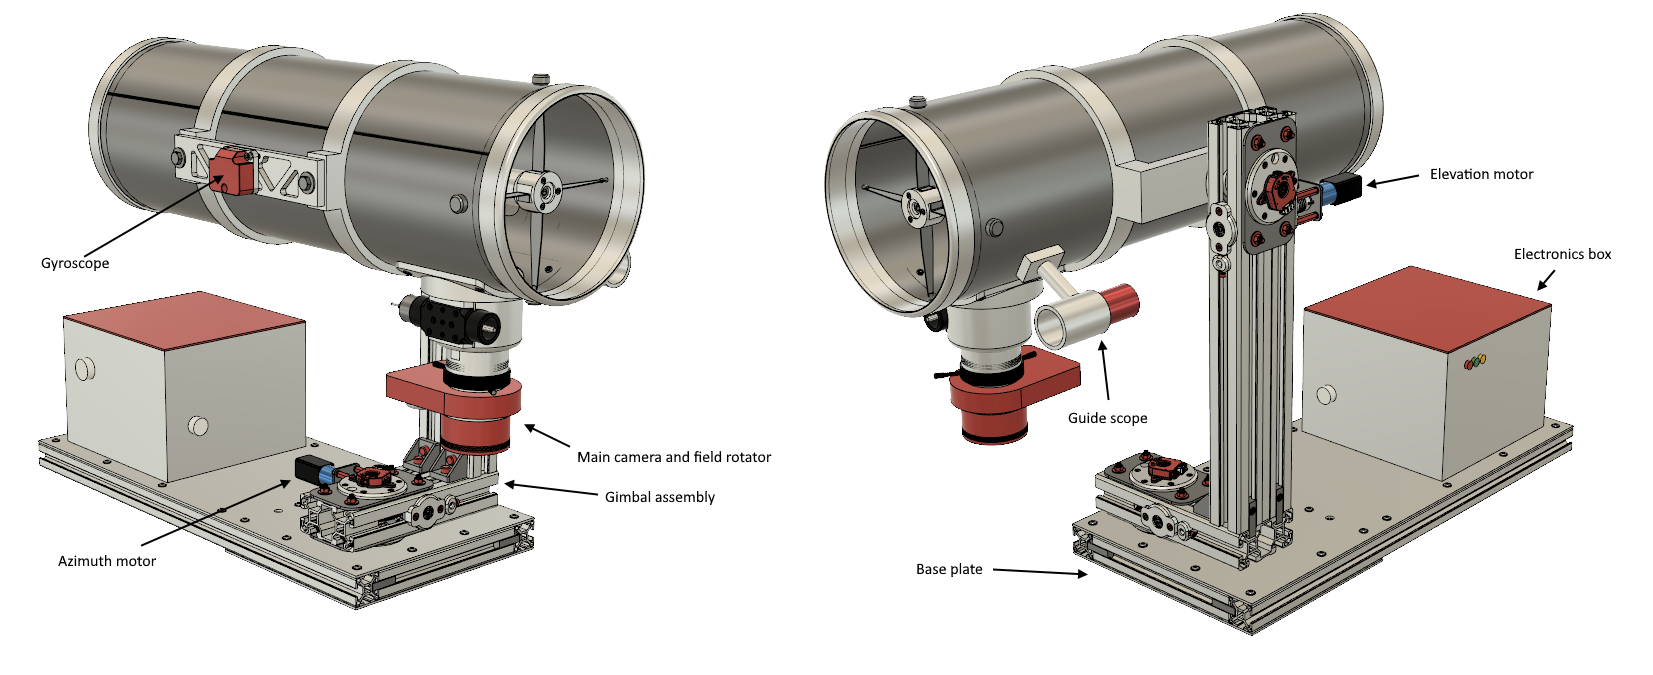
\includegraphics[width=\textwidth]{figures/Mechanical/iso1.png}
		\caption{Overall view of the experiment}	
		\label{img::mech1}
	\end{figure}
\end{frame}
\begin{frame}{Transmission}
	\begin{columns}[t]
		\begin{column}{0.45\textwidth}
			\begin{figure}
				\centering
				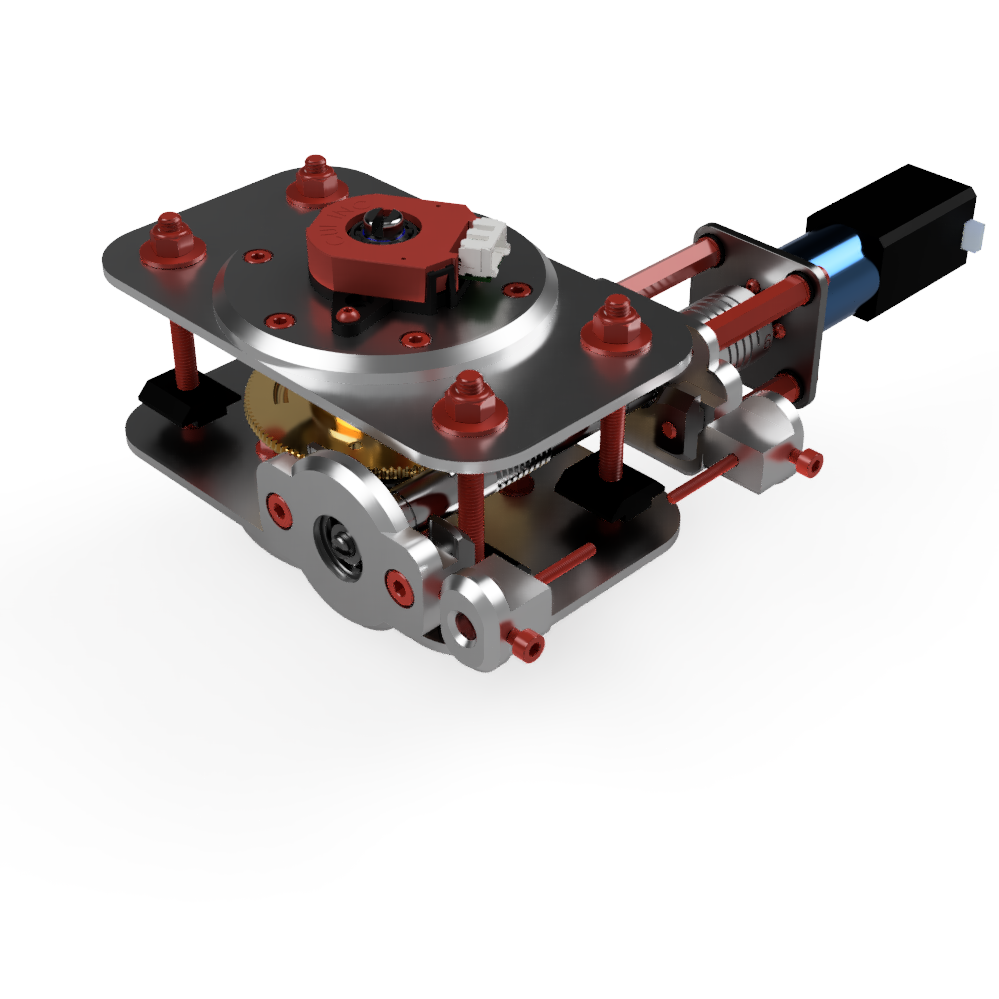
\includegraphics[width=\textwidth]{figures/Mechanical/transmission.png}
				\caption{Isometric view of the transmission}
				\label{img::mech2}
			\end{figure}
		\end{column}
		\begin{column}{0.45\textwidth}
			\begin{figure}
				\centering
				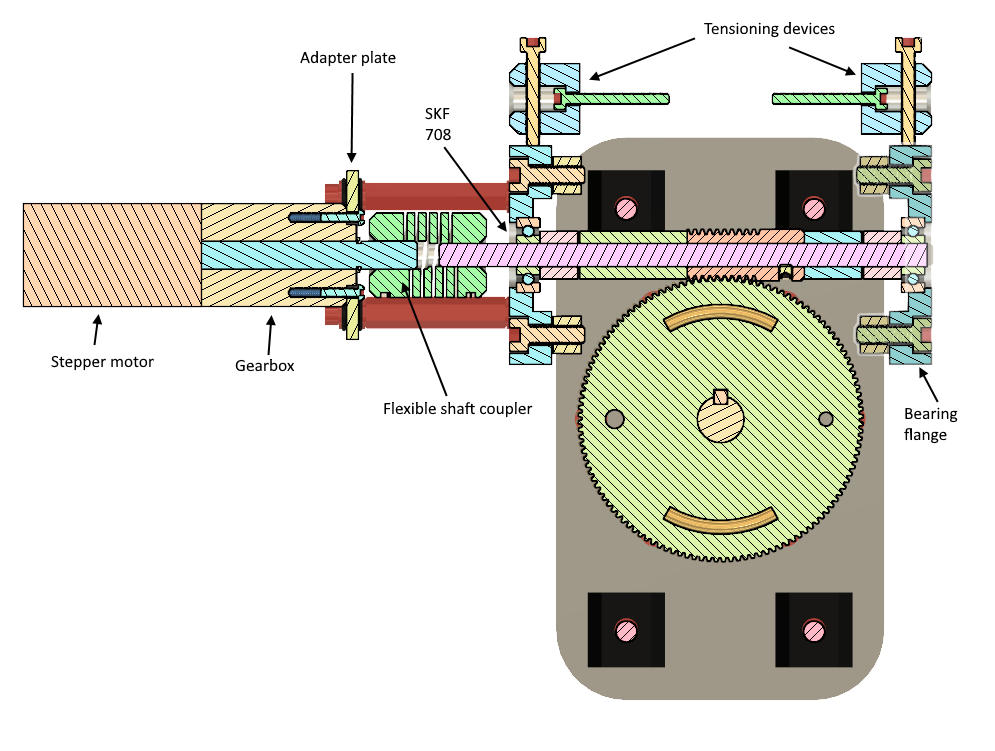
\includegraphics[width=\textwidth]{figures/Mechanical/Wormshaft_CS.png}
				\caption{Cross section of the transmission}
				\label{img::mech3}
			\end{figure}
		\end{column}
	\end{columns}

\end{frame}

%   THERMAL. ----------------------------------------------------------------------------

\subsection{Thermal}


%   ELECTRICAL. -------------------------------------------------------------------------
\subsection{Electrical Setup}

  \begin{frame}[c]{Electrical - Power}
    \begin{columns}[t]
        \begin{column}{.4\textwidth}
            \centering
            New components:
            \begin{itemize}
            	\item THN 30-2411WI - 5V, 6A, 30W\\ 
            	\item THN 30-4112WI -12V, 2.5A, 30W \\ 
            	\item NCP1117 - 3V3, voltage regulator with an input of 5A\\
            \end{itemize}
           
            RC filter will be used after the power supply components. 
        \end{column}
        \begin{column}{.6\textwidth}
        	\centering
        	\vspace{-.5cm}
            \begin{figure}
                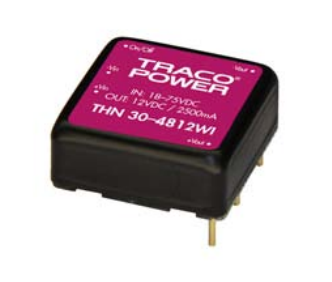
\includegraphics[scale=0.3]{component/tracoPowerComp.png}
                \caption{THN 30-2411WI - Power Supply Component.}
            \end{figure}
        \end{column}
    \end{columns}   
   \end{frame}


%   SOFTWARE. ---------------------------------------------------------------------------
\subsection{Software}

\begin{frame}[c]{Software - Current Status}
    \begin{itemize}
        \item Cameras
        \item Sensors
        \item E-Link Communications
        \item Data Handling
        \item Timeline of Events
        \item Control System
    \end{itemize}
\end{frame}

\begin{frame}[c]{Software - Cameras}
    \begin{columns}[t]
        \begin{column}{.4\textwidth}
            \begin{itemize}
                \item Finished
                \item Tested
                \item Upgrade to USB 3 needed
            \end{itemize}
        \end{column}
        
        \begin{column}{.6\textwidth}
            \begin{figure}[H]
                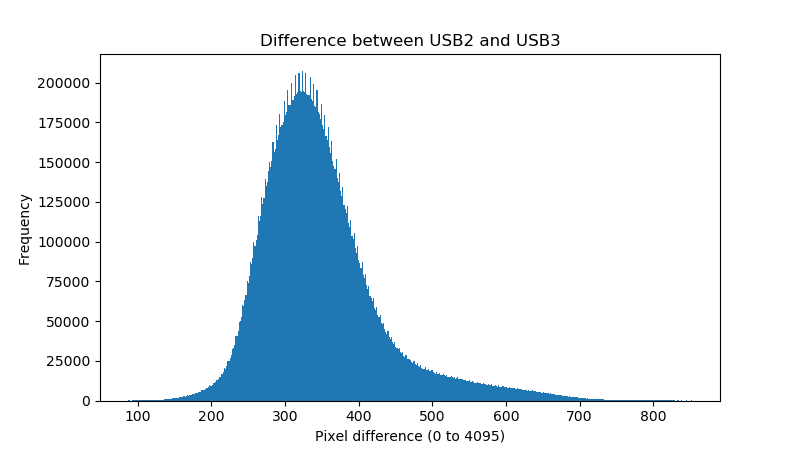
\includegraphics[width=\textwidth]{software/usb_comp.png}
                \caption{Comparison between USB 2 and 3 for the NIR camera}
            \end{figure}
        \end{column}
    \end{columns}
\end{frame}

\begin{frame}[c]{Software - Sensors}
    \begin{itemize}
        \item GPS: finished \& tested
        \item Encoders: finished
        \item IMU: implementation phase
        \item Star Tracker: implementation phase
    \end{itemize}
\end{frame}

\begin{frame}[c]{Software - E-Link Communications}
    \begin{itemize}
        \item Localhost
        \item Downlink: close to finished
        \item Uplink: implementation phase
        \item Commands: not yet started
    \end{itemize}
\end{frame}

\begin{frame}[c]{Software - Data Handling}
    \begin{itemize}
        \item Compression: finished
        \item Queuing: not yet started
        \item Sensor data logging: not yet started
    \end{itemize}
\end{frame}

\begin{frame}[c]{Software - Timeline of Events}
    \begin{itemize}
        \item Initialisation sequence: implementation phase
        \item Ascent phase: not yet started
        \item Start of float phase: not yet started
        \item Shutdown: not yet started
    \end{itemize}
\end{frame}

\begin{frame}[c]{Software - Current Issues}
    \begin{columns}[t]
        \begin{column}{.4\textwidth}
            \begin{itemize}
                \item Lack of library support for multiple buses on the Raspberry Pi 4B
                \item Encoders pull the data line high
            \end{itemize}
        \end{column}
        
        \begin{column}{.6\textwidth}
            \begin{figure}[H]
                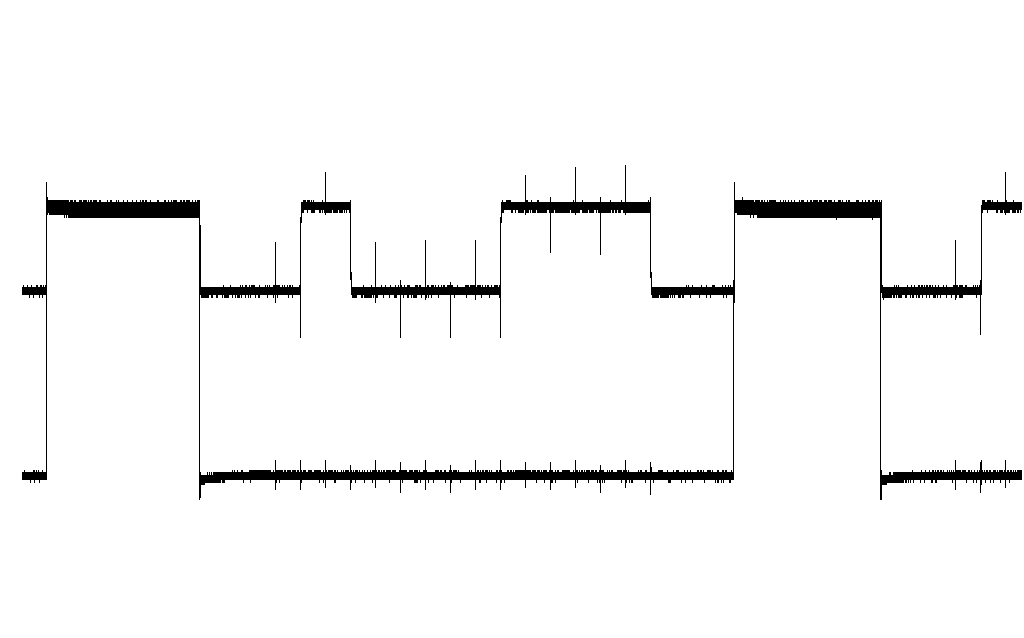
\includegraphics[width=\textwidth]{software/encoder_gps_bus.png}
                \caption{Encoders interfering with data sent from GPS receiver}
            \end{figure}
        \end{column}
    \end{columns}
\end{frame}

\subsection{Telescope and Cameras}

%----------------------------------------------------------------------------------------
%   PROJECT MANAGEMENT.
%----------------------------------------------------------------------------------------
\section{Project Management}
%   TEAM. ---------------------------------------------------------------------------
\subsection{Team composition}
\subsection{Project schedule}

%   BUDGET. -----------------------------------------------------------------------------
\subsection{Budget}
    
    %   OUTREACH. ---------------------------------------------------------------------------
\subsection{Outreach}


%----------------------------------------------------------------------------------------
%   SUMMARY.
%----------------------------------------------------------------------------------------
\section{Summary}

%----------------------------------------------------------------------------------------
%   QUESTIONS.
%----------------------------------------------------------------------------------------
\section{Questions}
%----------------------------------------------------------------------------------------
%   BACKUP SLIDES.              EVERYONE!!!
%----------------------------------------------------------------------------------------
\end{document}
